This chapter lists the requirements for the effects presented in the analysis. 

\begin{figure}[htbp]
	\centering
\begin{picture}(0,0)%
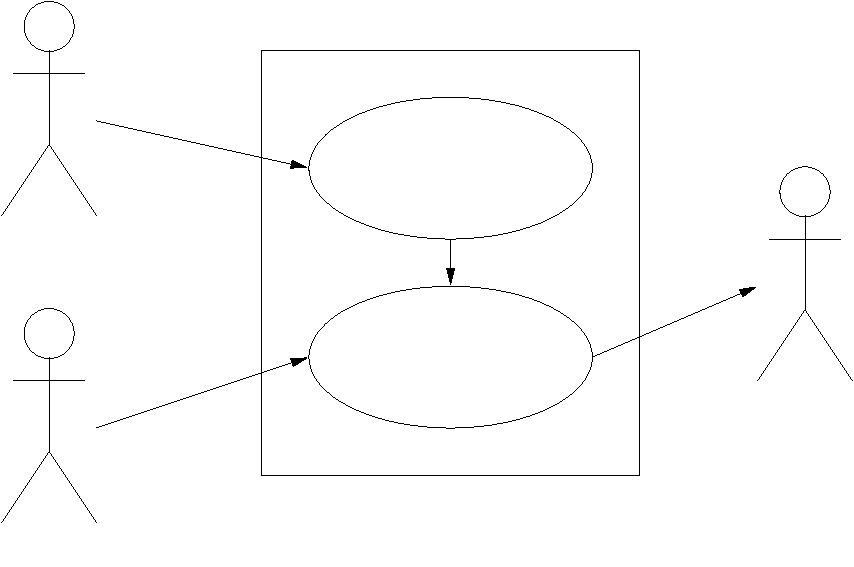
\includegraphics{Use_case.pdf}%
\end{picture}%
\setlength{\unitlength}{4144sp}%
%
\begingroup\makeatletter\ifx\SetFigFont\undefined%
\gdef\SetFigFont#1#2#3#4#5{%
  \reset@font\fontsize{#1}{#2pt}%
  \fontfamily{#3}\fontseries{#4}\fontshape{#5}%
  \selectfont}%
\fi\endgroup%
\begin{picture}(6507,4318)(1426,-4900)
\put(1531,-2491){User}%
\put(4546,-3346){Effect}%
\put(4276,-1906){Effect select}%
\put(7111,-3751){Amplifier}%
\put(1441,-4831){Guitar}%
\end{picture}%
	\caption{A graphically overview of wanted functionality in form of an use case digram.}
	\label{fig:use_case}
\end{figure}

From \autoref{ch:analysing_cl} it is seen that some of the effects can be designed together, because the effects use the same parts but multiple times or with a small modification. The following description tells shortly about the difference in the effect blocks and which effect that can be designed together.

\paragraph*{Basic filtering}
The only basis filter explained in \autoref{ch:analysing}, which is a basic filter without delay or frequency scaling, is the Equalizer.

\paragraph{Frequency scaling filter}
The only frequency scaling filter explained in \autoref{ch:analysing} is the Wah-Wah.

\paragraph{Delay}
All the delay based effects have at least one delay block and have both fast and slow delay. All the analysed delayed based effects in \autoref{ch:analysing} are:
\begin{itemize}
	\item Delay
	\item \gls{reverb}
	\item Flanger
	\item Chorus
\end{itemize} 

The block diagram in each effect shows that pair wise effects have a common structure. The chorus is the flanger with the same effect added more than once. The same is the case for delay and \gls{reverb} respectively. Then the only two effect which needed to be designed is Chorus and \gls{reverb} because Flanger and Delay can easily be made by removing the multiply parts in their respective effect.

\paragraph{Non-linear processing}
\begin{itemize}
	\item Distortion
	\item Overdrive
\end{itemize} 

\subsection{Block}

The requirements are divided into units, based on the effect analysis \autoref{ch:analysing}, since it is concluded in \autoref{ch:analysing_cl} that only six general units need to be designed and all the presented effects can be created from these. The units that are going to be designed are the:



\begin{itemize}
	\item Bandpass filter
	\item Inverse bandpass filter
	\item Delay
	\item Gain
	\item Clipping
	\item \gls{lfo}
\end{itemize} 

 Besides the fact that each unit shall be designed individually, each unit interface should fit in the effect that is using it. Each unit has its own section where the requirements and their arguments are presented. To ensure that the units can fit and work together, basic requirements  are made to the processing component.
 
 